\chapter{System Build and Estimation}
\label{ch:estimation}

A feature map and a classifier become a diagnosis only when a machine, a sensor, and a clock produce the records they assume.
This chapter specifies that build from the published rig description, then estimates the pair of technologies on the published classification counts.
The estimate is a reading of a completed experiment.
It is not a new acquisition.

\section{Construction of the diagnostic system}
\label{sec:build}

\subsection{The hydraulic loop and the machine}

The rotating machine is a vertical axial-flow pump in a closed water loop.
The pump drives water around the circuit, so the hydraulic load exists for the whole record and does not depend on an external consumer.
Table~\ref{tab:rig} collects the operating point stated in the source.
The rotational speed is \(960\,\mathrm{r/min}\), the flow is \(550\,\mathrm{m}^{3}/\mathrm{h}\), the head is \(3\,\mathrm{m}\), and the impeller has four blades.
From the speed alone, equation \eqref{eq:f0} fixes the shaft rate at \(16\,\mathrm{Hz}\).
From the blade count, equation \eqref{eq:bpfreq} fixes blade pass at \(64\,\mathrm{Hz}\).
The head and the flow fix the duty, which matters because a seal-wear fault is a leakage superimposed on this duty, not a dry mechanical defect.
A reader who repeats the experiment at a different flow should expect the hydraulic features, especially the seal-wear pattern and the high-order axial energy, to move.

\begin{table}[H]
\centering
\caption{Published operating point of the vertical axial-flow pump.}
\label{tab:rig}
\begin{tabular}{ll}
\toprule
Quantity & Value \\
\midrule
Machine & Vertical axial-flow pump \\
Rotational speed & \(960\,\mathrm{r/min}\) \\
Shaft frequency \(f_{0}\) & \(16\,\mathrm{Hz}\) \\
Flow rate & \(550\,\mathrm{m}^{3}/\mathrm{h}\) \\
Head & \(3\,\mathrm{m}\) \\
Impeller blade count \(Z\) & \(4\) \\
Blade-pass frequency \(Z f_{0}\) & \(64\,\mathrm{Hz}\) \\
Installation & Closed water loop \\
\bottomrule
\end{tabular}
\end{table}

The loop has a water inlet and a water outlet at the pump, a triaxial accelerometer on the casing, and the pump body itself as the dominant structure in the measurement path.
Figure~\ref{fig:rig} is a schematic of that arrangement.
It is not a dimensioned drawing of the laboratory.
The accelerometer sits on the pump so that casing motion, rather than pipe-wall motion far from the rotor, is what enters \(\Phi\).
Pipe vibration would still be present in the background, and the source attributes part of the high-order energy under the pedestal fault to flow-induced vibration of internal components.
The schematic keeps the sensor on the machine because that is the path the severities were measured on.

\begin{figure}[H]
\centering
\begin{tikzpicture}[
  blk/.style={draw, rounded corners=2pt, align=center, font=\small, inner sep=3pt, minimum height=9mm},
  arr/.style={-{Stealth[length=2.2mm]}, thick}
]
  \node[blk, fill=blue!10, text width=28mm] (in) {Water inlet};
  \node[blk, fill=blue!18, text width=34mm, right=8mm of in] (pump) {Vertical axial-flow\\pump, \(960\,\mathrm{r/min}\)};
  \node[blk, fill=blue!10, text width=28mm, right=8mm of pump] (out) {Water outlet};
  \node[blk, fill=orange!15, text width=32mm, below=8mm of pump] (sen) {Triaxial charge\\accelerometer};
  \node[blk, fill=orange!15, text width=36mm, below=6mm of sen] (pxi) {Charge amplifiers\\and PXI acquisition};
  \node[blk, fill=green!12, text width=36mm, below=6mm of pxi] (pc) {VWC map and\\MSFLA-SVM};
  \draw[arr] (in) -- (pump);
  \draw[arr] (pump) -- (out);
  \draw[arr, dashed] (out.south) -- ++(0,-1.55) -| (in.south);
  \node[font=\scriptsize] at (4.55,-1.15) {closed loop};
  \draw[arr] (pump) -- (sen);
  \draw[arr] (sen) -- (pxi);
  \draw[arr] (pxi) -- (pc);
\end{tikzpicture}
\caption{Schematic of the diagnostic build. The dashed path is the closed water loop. The solid vertical path is the measurement and decision chain.}
\label{fig:rig}
\end{figure}

\subsection{The four operating states and how they are produced}

The experiment defines four mutually exclusive states.
The healthy state is the pump at the duty of Table~\ref{tab:rig} with no intentional defect.
The other three states are produced by a physical change, not by a numerical simulation.

Eccentric-axle fault is produced by moving a weight on the shaft so that the mass center leaves the geometric axis.
In the language of \eqref{eq:rotor} the change is an increase of the unbalance \(m e\).
The expected stationary signature is a rise of the force at \(f_{0}\) and, because severity integrates velocity rather than a single Fourier coefficient, a rise of VIB.
Both are observed: severity goes from \(1.051\) to \(3.737\,\mathrm{mm/s}\), and the tangential coefficient spectrum peaks at \(f_{0}\) with a larger amplitude than in the healthy state.
The source also notes energy at \(28\), \(34\), and \(38\,\mathrm{Hz}\) and attributes it to crosstalk from other devices in the laboratory.
Those tones are not members of \(\mathcal{F}\).
A feature map that sampled only \(\mathcal{F}\) is, by design, partly protected from them, and a feature map that used the whole spectrum as a long vector would have to learn to ignore them from forty-five training records.
This is one practical reason the \(22\)-vector is short.

Bearing-pedestal fault begins in the rolling-element bearing and is observed at the pedestal that supports it.
The source describes the usual bearing sequence: fatigue, wear, and adhesion, followed by a periodic jump of the pedestal, a change of the support stiffness, and an impact.
The expected spectral signature of a stiffness that is not constant inside one revolution includes a half-order line.
The published reading matches that expectation in the tangential direction, where the coefficient spectrum peaks at \(\tfrac12 f_{0}=8\,\mathrm{Hz}\).
Severity barely moves, from \(1.051\) to \(1.161\,\mathrm{mm/s}\).
The pedestal state is therefore a shape fault rather than an intensity fault, which is why it is included.
A rig that only seeded unbalance would let severity do the classification and would not test VWC.

Sealing-ring wear is a degradation of the ring that limits backflow from the discharge side and that keeps the impeller from rubbing the casing.
Wear opens a leakage path and risks impeller damage.
The expected signature is a hydraulic load at shaft order and at twice shaft order, together with a half-order component from the resulting asymmetry.
The published reading again matches: severity rises to \(1.70024\,\mathrm{mm/s}\), intermediate between the healthy and the eccentric states, and the spectrum emphasizes \(f_{0}\), \(\tfrac12 f_{0}\), and \(2f_{0}\).
The tangential direction carries the largest amplitudes, as it does in the other three states.

The four states are run as four separate conditions.
The published study does not include mixed faults, a slow ramp from healthy to faulty, or a speed sweep.
The classifier is therefore a four-way state identifier at one duty point.
Extending it to mixed faults would require a new sample and a decision about whether the label set stays a partition.

\subsection{The sensor and the three directions}

The transducer is a B\&K~4321 triaxial charge accelerometer.
Table~\ref{tab:sensor} lists the characteristics the source prints.
The charge sensitivity is \(9.8\,\mathrm{pC/g}\) within \(\pm 2\%\), which is approximately one picocoulomb per metre per second squared, because standard gravity is \(9.81\,\mathrm{m/s}^{2}\).
The stated frequency range, \(0.1\,\mathrm{Hz}\) to \(12\,\mathrm{kHz}\), covers the shaft family and the resonances that dominate acceleration.
The amplitude range is \(500\,g\).
The time-domain plots in the source have peaks of roughly \(7\) to \(9\,\mathrm{m/s}^{2}\), about one \(g\), so the records sit far below the range limit and clipping is not the explanation of any class error.

\begin{table}[H]
\centering
\caption{Published transducer and acquisition parameters.}
\label{tab:sensor}
\begin{tabular}{lll}
\toprule
Element & Parameter & Value \\
\midrule
B\&K 4321 & Type & Triaxial charge accelerometer \\
 & Charge sensitivity & \(9.8\pm 2\%\,\mathrm{pC/g}\) \\
 & Frequency range & \(0.1\) to \(12\,000\,\mathrm{Hz}\) \\
 & Measuring range & \(500\,g\) \\
\midrule
PXI acquisition card & Sampling frequency & \(100\,\mathrm{Hz}\) to \(100\,\mathrm{kHz}\), set to \(10\,\mathrm{kHz}\) \\
 & Input channels & \(8\) \\
 & Input range & \(\pm 100\,\mathrm{mV}\) to \(\pm 10\,\mathrm{V}\) \\
 & Stated precision & \(\pm 0.1\%\) of full-scale range, DC \\
\bottomrule
\end{tabular}
\end{table}

Charge leaves the sensor and enters a charge amplifier, whose voltage output is sampled by a PXI card with eight input channels, a selectable range from \(\pm 100\,\mathrm{mV}\) to \(\pm 10\,\mathrm{V}\), and a stated DC accuracy of \(\pm 0.1\%\) of full scale.
Three of the eight channels are required, one per axis.
The card can sample at up to \(100\,\mathrm{kHz}\); the experiment sets \(10\,\mathrm{kHz}\).
The Nyquist frequency is therefore \(5\,\mathrm{kHz}\).
The sensor itself responds up to \(12\,\mathrm{kHz}\), which is above Nyquist, so an anti-alias filter before the converter is part of a correct build.
The source table does not list that filter.
A repetition of the rig should place the filter cutoff below \(5\,\mathrm{kHz}\) with a stopband that covers the sensor's remaining bandwidth, and should record the cutoff next to the sampling rate.
Without it, energy between \(5\) and \(12\,\mathrm{kHz}\) folds into the analysis band and can move both the winning wavelet level and the high-order amplitudes.

The three axes are radial, tangential, and axial relative to the vertical rotor.
Figure~\ref{fig:axes} names them.
Unbalance forces lie in the plane perpendicular to the shaft, so they drive the radial and tangential channels.
A vertical hydraulic load drives the axial channel.
The published coefficient spectra say that the tangential channel has the largest amplitudes in every state.
Keeping all three is still necessary, because the axial channel is where the pedestal fault shows the high-order growth at \(5f_{0}\) and \(6f_{0}\), and the radial channel is where the published severity is defined.

\begin{figure}[H]
\centering
\begin{tikzpicture}[>=Stealth, thick]
  \draw[->] (0,0) -- (3.1,0) node[right] {tangential};
  \draw[->] (0,0) -- (0,3.1) node[above] {axial (vertical shaft)};
  \draw[->] (0,0) -- (2.1,1.5) node[above right] {radial};
  \fill (0,0) circle (1.6pt);
  \node[font=\small, align=left] at (4.6,1.4) {Sensor axes on the casing.\\Shaft frequency \(16\,\mathrm{Hz}\).\\Blade pass \(64\,\mathrm{Hz}\) along\\the rotating load.};
\end{tikzpicture}
\caption{The three measurement directions. The feature vector repeats the seven shaft-order amplitudes once in each direction and appends the radial severity.}
\label{fig:axes}
\end{figure}

\subsection{Sampling arithmetic}

Several numbers that the later estimate depends on are fixed by the clock and the record length, and they are worth writing once.
The sampling rate is \(f_{s}=10^{4}\,\mathrm{Hz}\).
The analysis length used to describe the records is \(N=8192\) samples, which is the right edge of the time-domain plots in the source.
The duration, the frequency resolution of a full-length Fourier transform, the number of shaft revolutions inside the record, and the Nyquist frequency are
\begin{align}
T_{\mathrm{rec}}&=\frac{N}{f_{s}}=\frac{8192}{10000}=0.8192\,\mathrm{s},&
\Delta f&=\frac{f_{s}}{N}=1.2207\,\mathrm{Hz},\\
N_{\mathrm{rev}}&=T_{\mathrm{rec}} f_{0}=13.107,&
f_{\mathrm{Nyq}}&=\frac{f_{s}}{2}=5\,\mathrm{kHz}.
\label{eq:arith}
\end{align}
Thirteen revolutions are enough for a stable estimate of a once-per-revolution line and are short enough that a pedestal impact does not have to be stationary over a long average.
The resolution \(1.2207\,\mathrm{Hz}\) puts \(3f_{0}=48\,\mathrm{Hz}\) and the supply line at \(50\,\mathrm{Hz}\) in different bins, with a gap of \(1.64\) bins.
An order sampler aimed at \(48\,\mathrm{Hz}\) with a half-order acceptance window of \(4\,\mathrm{Hz}\), as specified in Section~\ref{sec:vwc}, does not include \(50\,\mathrm{Hz}\).
That exclusion is deliberate.
It is also a limitation: a real supply harmonic that modulates a mechanical line inside the window will still be admitted.

At level \(j\) of a dyadic bank the coefficient rate is \(f_{s}/2^{j}\) and the length of the coefficient sequence is about \(N/2^{j}\).
For the level the source plots, \(j=5\), the coefficient rate is \(312.5\,\mathrm{Hz}\) and the coefficient record contains \(256\) samples.
A Fourier transform of those coefficients has a bin spacing of \(312.5/256=1.2207\,\mathrm{Hz}\), the same spacing as the full-length transform of the original record, and a coefficient-domain Nyquist of \(156.25\,\mathrm{Hz}\).
Every member of \(\mathcal{F}\), including \(6f_{0}=96\,\mathrm{Hz}\), lies inside that coefficient-domain Nyquist frequency.
The seven-order sampler is therefore well defined on \(d_{5}\) without a further resampling.
Had the winning level been \(d_{3}\), the coefficient Nyquist would have been \(625\,\mathrm{Hz}\) and the same orders would still lie inside it, with coarser relative localization.
Had the winning level been deeper than \(d_{7}\), the coefficient Nyquist would fall below \(96\,\mathrm{Hz}\) and \(6f_{0}\) would cease to be observable at that level.
The maximum-energy rule can in principle select such a level.
On the records the source plots, it selects \(d_{5}\), where all seven orders are observable.
An implementation should refuse an order that sits above the coefficient Nyquist of \(k^{\star}\) and should record the refusal, rather than report a folded frequency as if it were \(6f_{0}\).

\subsection{Sample size, split, and the unit of analysis}

The source collects \(60\) groups of data in each of the four states, \(240\) groups in all.
Each group is one \(22\)-vector.
Forty-five groups per state are the training sample and fifteen are the test sample, so the design matrices have shapes
\begin{equation}
\vect{X}_{\mathrm{train}}\in\R^{180\times 22},
\qquad
\vect{X}_{\mathrm{test}}\in\R^{60\times 22}.
\label{eq:shapes}
\end{equation}
The split is stratified by construction: each state contributes the same count to each matrix.
The source does not say whether the fifteen test groups were drawn at random, taken from the end of each run, or chosen by hand.
A repetition should draw them at random inside each state and should freeze the draw before any search over \((C, g)\).
Because the search described in Section~\ref{sec:svm} uses cross-validation inside the training matrix only, the sixty test rows are available for a single estimate.

Sixty test vectors is a small denominator.
One misclassified test vector moves a per-class rate by \(1/15\approx 6.67\) percentage points and moves the pooled rate by \(1/60\approx 1.67\) percentage points.
The difference between MSFLA-SVM and SFLA-SVM on the test set is one vector in the pooled count (\(56\) against \(55\)).
That difference is real as a count and it is small as evidence.
Section~\ref{sec:estimate} reports it as a count.

The source remarks that more records could not be collected under the conditions of the experiment, and that the SVM is used precisely because the sample is small.
The system build should be read with that constraint in view.
The acquisition is adequate for a four-class comparison at one duty.
It is not a durability test, and it is not a variable-speed campaign.

\subsection{The processing path}

Figure~\ref{fig:path} assembles the path from a stored record to a label.
The same path produces the training matrix and, with the normalization frozen, the test matrix.
Baselines branch after the normalization.
They do not receive a different feature.

The backpropagation baseline is the network of the kind Huang and Xie trained for bearing diagnosis~\cite{huang2009}, used here as the source uses it: a nonlinear classifier of the \(22\)-vector with no frog search.
The ACROA-SVM baseline is the radial SVM with parameters proposed by the artificial chemical reaction search of Alatas, in the bearing configuration of Ao, Cheng, Li, and Truong~\cite{ao2014,alatas2011}.
The SFLA-SVM baseline is the same radial SVM with the unmodified leap of Section~\ref{sec:svm}.
MSFLA-SVM is the modified leap.
All four see \(\tilde{\vect{x}}\) from \eqref{eq:norm}.
This common front end is what makes the table an estimate of classifiers rather than an estimate of features.
The source does not publish an ablation that removes severity, or the half-order, or one of the axes.
The present reading therefore cannot say which of the twenty-two coordinates carries the pedestal separation.
It can say that the full vector, shared by four classifiers, is sufficient for a pooled test accuracy above \(90\%\) for every SVM variant and not for the neural baseline.

\begin{figure}[H]
\centering
\begin{tikzpicture}[
  box/.style={draw, rounded corners=2pt, align=center, font=\small, inner sep=2.5pt, minimum height=8mm},
  arr/.style={-{Stealth[length=2mm]}, thick}
]
\node[box, fill=blue!8, text width=30mm] (rec) {Stored triaxial\\records, four states};
\node[box, fill=orange!12, text width=28mm, right=5mm of rec] (phi) {VWC map\\\(\Phi\)};
\node[box, fill=orange!12, text width=26mm, right=5mm of phi] (sc) {Scale on\\training ranges};
\node[box, fill=gray!10, text width=22mm, below=7mm of sc] (bp) {BPNN};
\node[box, fill=gray!10, text width=24mm, left=3mm of bp] (ac) {ACROA-SVM};
\node[box, fill=gray!10, text width=24mm, left=3mm of ac] (sf) {SFLA-SVM};
\node[box, fill=green!15, text width=26mm, left=3mm of sf] (ms) {MSFLA-SVM};
\node[box, fill=green!18, text width=24mm, below=7mm of ac] (lab) {Label in \(\mathcal{Y}\)};
\draw[arr] (rec) -- (phi);
\draw[arr] (phi) -- (sc);
\draw[arr] (sc) -- (bp);
\draw[arr] (sc.south) ++(-0.2,0) -- ++(0,-0.35) -| (ac.north);
\draw[arr] (sc.south) ++(-0.2,0) -- ++(0,-0.55) -| (sf.north);
\draw[arr] (sc.south) ++(-0.2,0) -- ++(0,-0.75) -| (ms.north);
\draw[arr] (ms) -- (lab);
\draw[arr] (sf) -- (lab);
\draw[arr] (ac) -- (lab);
\draw[arr] (bp) -- (lab);
\end{tikzpicture}
\caption{Processing path. The four classifiers are interchangeable blocks after a shared, train-scaled VWC vector.}
\label{fig:path}
\end{figure}

\subsection{What the build guarantees and what it leaves open}

The build guarantees a constant speed, a constant hydraulic duty, a triaxial casing measurement, a sampling rate that places the shaft family and the supply line on a resolvable grid, a record long enough for about thirteen revolutions, and a stratified sample of sixty vectors per state.
It leaves open the mother wavelet, the exact integrator inside the published severity, the anti-alias cutoff, the random seed of the split, and the population parameters of every evolutionary search.
Chapter~\ref{ch:methods} specified the wavelet, the normalization, the coding of the four classes, and the box of \((C, g)\) for this exposition, and it refused to invent the unpublished population parameters.
The estimate in the next section is attached to the source's run, under the source's unpublished choices, and the numerical values are taken from the source's tables.

\section{Estimation of diagnostic performance}
\label{sec:estimate}

\subsection{Signatures of the four states}
\label{sec:signatures}

The qualitative estimate comes before the percentages, because a classifier that scores well on a feature with no mechanical reading is a different claim from a classifier that scores well on VWC.
Table~\ref{tab:sign} compresses the source's reading of its time-domain records, its coefficient spectra, and its energy time-spectra.
Every state has its maximum wavelet energy at the \(d_{5}\) level in the radial plots the source prints.
The states differ in severity and in which member of \(\mathcal{F}\) dominates the tangential coefficient spectrum.

\begin{table}[H]
\centering
\caption{Published qualitative signatures of the four states, radial severity and tangential spectral emphasis.}
\label{tab:sign}
\small
\begin{tabular}{p{2.4cm}p{2.3cm}p{3.6cm}p{4.6cm}}
\toprule
State & Radial severity & Dominant tangential orders & Notes published with the records \\
\midrule
Normal & \(1.051\,\mathrm{mm/s}\) & \(f_{0}\), then \(2f_{0}\), \(3f_{0}\) & Supply line at \(50\,\mathrm{Hz}\); blade-pass energy at \(4f_{0}=64\,\mathrm{Hz}\). \\
EAF & \(3.737\,\mathrm{mm/s}\) & \(f_{0}\) & Crosstalk at \(28\), \(34\), and \(38\,\mathrm{Hz}\). Largest severity of the four states. \\
BPF & \(1.161\,\mathrm{mm/s}\) & \(\tfrac12 f_{0}\), with \(f_{0}\) and \(3f_{0}\) & High-order axial growth at \(5f_{0}\) and \(6f_{0}\), attributed to flow and to component natural frequencies. \\
SRWF & \(1.700\,\mathrm{mm/s}\) & \(f_{0}\), \(\tfrac12 f_{0}\), \(2f_{0}\) & Tangential energy is the largest; axial and radial intensities lie between EAF and BPF. \\
\bottomrule
\end{tabular}
\end{table}

A few published amplitudes make the tangential dominance quantitative.
Healthy tangential peak coefficient power is \(1.683\times 10^{-3}\) at \(f_{0}\).
Eccentric tangential peak power is \(3.322\times 10^{-3}\).
Pedestal tangential peak power is \(4.701\times 10^{-3}\) at \(\tfrac12 f_{0}\).
Healthy radial peak power is \(4.574\times 10^{-4}\), and eccentric radial peak power is \(2.492\times 10^{-3}\).
The pedestal tangential peak is about \(2.8\) times the healthy tangential peak, while the pedestal severity is only \(1.10\) times the healthy severity.
The spectral coordinate moves by a larger factor than the severity coordinate.
That comparison is the empirical reason the \(22\)-vector contains both, and the reason a severity threshold is not a substitute for the classifier.

The illustrative spectra in Figure~\ref{fig:spectra} were drawn to carry the same emphasis: healthy and eccentric energy at \(f_{0}\), pedestal and seal-wear energy with a stronger half-order.
They should be used as a picture of the emphasis and not as a source of amplitudes.
The amplitudes in the previous paragraph are the ones the source prints.

\subsection{Training estimate}

Training accuracy is the accuracy of each finished classifier on the \(180\) vectors it was trained on.
For the three SVM methods the finished classifier is the machine retrained on all \(180\) rows at the \((C, g)\) the search returned, so the training accuracy is an in-sample number and is expected to sit above the cross-validated fitness that guided the search.
Table~\ref{tab:train} gives the count of correct training vectors.
The percentages are those counts divided by \(45\), except where a printed percentage in the source decides an inconsistent count; the training table is internally consistent, and no such correction is required.
Each row average is the unweighted mean of the four method percentages, matching the source.
Each column average at the foot is the pooled accuracy, correct counts summed over states and divided by \(180\).

\begin{table}[H]
\centering
\caption{Training classification counts on \(45\) vectors per state. Pooled accuracy is correct-over-\(180\).}
\label{tab:train}
\begin{tabular}{lrrrrr}
\toprule
State & BPNN & ACROA-SVM & SFLA-SVM & MSFLA-SVM & Row mean \\
\midrule
Normal & 42/45 & 45/45 & 45/45 & 45/45 & 98.333\% \\
 & 93.333\% & 100\% & 100\% & 100\% & \\
EAF & 41/45 & 44/45 & 43/45 & 45/45 & 96.111\% \\
 & 91.111\% & 97.778\% & 95.556\% & 100\% & \\
BPF & 40/45 & 42/45 & 42/45 & 43/45 & 92.778\% \\
 & 88.889\% & 93.333\% & 93.333\% & 95.556\% & \\
SRWF & 42/45 & 44/45 & 44/45 & 44/45 & 96.667\% \\
 & 93.333\% & 97.778\% & 97.778\% & 97.778\% & \\
\midrule
Pooled & 165/180 & 175/180 & 174/180 & 177/180 & \\
 & 91.667\% & 97.222\% & 96.667\% & 98.333\% & \\
\bottomrule
\end{tabular}
\end{table}

The source prints the MSFLA pooled training accuracy as \(98.334\%\).
The exact ratio \(177/180\) is \(98.333\ldots\%\).
The difference is rounding.
This paper uses the ratio.

Figure~\ref{fig:train} shows the same rates.
Three facts are visible without the figure.
The healthy state is the easiest training class for every method, and every SVM variant classifies all \(45\) healthy training vectors correctly.
The pedestal state is the hardest training class for every method: \(40\), \(42\), \(42\), and \(43\) correct out of \(45\).
MSFLA-SVM is the unique method that classifies all \(45\) eccentric training vectors correctly, and it is tied or ahead on every state.
Its pooled gain over SFLA-SVM is three training vectors (\(177\) against \(174\)).
Its pooled gain over the neural baseline is twelve training vectors.

\begin{figure}[H]
\centering
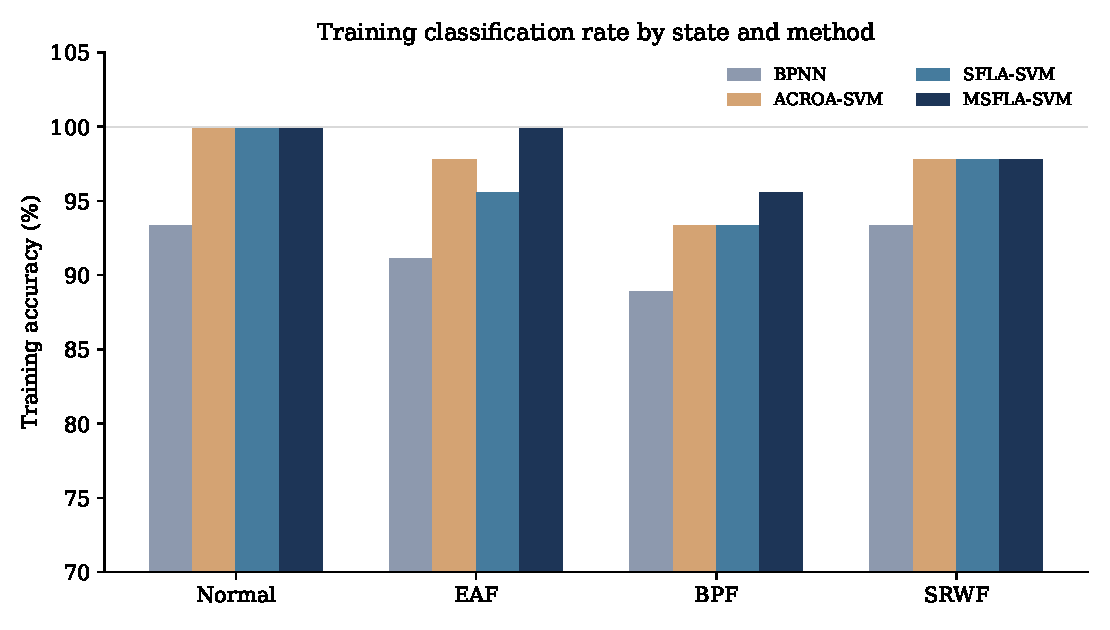
\includegraphics[width=0.92\textwidth]{train_accuracy.pdf}
\caption{Training accuracy by state and method, from Table~\ref{tab:train}.}
\label{fig:train}
\end{figure}

\subsection{Testing estimate}

Test accuracy is the quantity the search was not allowed to see.
Fifteen vectors per state, sixty in all, are labeled by the finished classifiers.
Table~\ref{tab:test} records the result.
For the backpropagation row of the sealing-ring state, the source prints a count of \(12/15\) beside a percentage of \(86.667\%\).
Those two entries disagree, because \(12/15=80\%\) and \(13/15=86.667\%\).
The four printed BPNN percentages \(86.667\), \(86.667\), \(80\), and \(86.667\) average to the printed pooled value \(85\%\), and the counts \(13\), \(13\), \(12\), and \(13\) sum to \(51\), with \(51/60=85\%\).
The count that agrees with the printed percentage and with the printed pooled accuracy is \(13/15\).
Table~\ref{tab:test} uses that count.
No other test cell requires a correction: ACROA, SFLA, and MSFLA are consistent with their pooled rates of \(91.667\%\), \(91.667\%\), and \(93.333\%\).

\begin{table}[H]
\centering
\caption{Test classification on \(15\) vectors per state. The BPNN entry for SRWF is \(13/15\), the count consistent with the printed percentage \(86.667\%\) and the printed pooled accuracy \(85\%\).}
\label{tab:test}
\begin{tabular}{lrrrrr}
\toprule
State & BPNN & ACROA-SVM & SFLA-SVM & MSFLA-SVM & Row mean \\
\midrule
Normal & 13/15 & 15/15 & 15/15 & 15/15 & 96.667\% \\
 & 86.667\% & 100\% & 100\% & 100\% & \\
EAF & 13/15 & 13/15 & 14/15 & 14/15 & 90.000\% \\
 & 86.667\% & 86.667\% & 93.333\% & 93.333\% & \\
BPF & 12/15 & 13/15 & 13/15 & 13/15 & 85.000\% \\
 & 80.000\% & 86.667\% & 86.667\% & 86.667\% & \\
SRWF & 13/15 & 14/15 & 13/15 & 14/15 & 90.000\% \\
 & 86.667\% & 93.333\% & 86.667\% & 93.333\% & \\
\midrule
Pooled & 51/60 & 55/60 & 55/60 & 56/60 & \\
 & 85.000\% & 91.667\% & 91.667\% & 93.333\% & \\
\bottomrule
\end{tabular}
\end{table}

\begin{figure}[H]
\centering
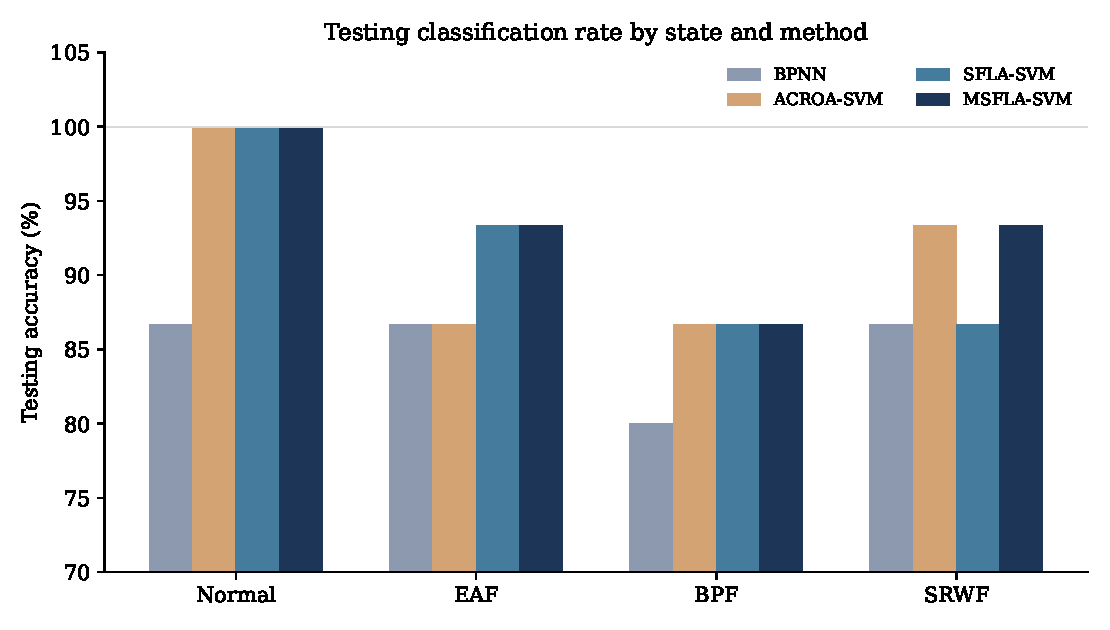
\includegraphics[width=0.92\textwidth]{test_accuracy.pdf}
\caption{Test accuracy by state and method, from Table~\ref{tab:test}. The pedestal state is the lowest bar in every group.}
\label{fig:test}
\end{figure}

\begin{figure}[H]
\centering
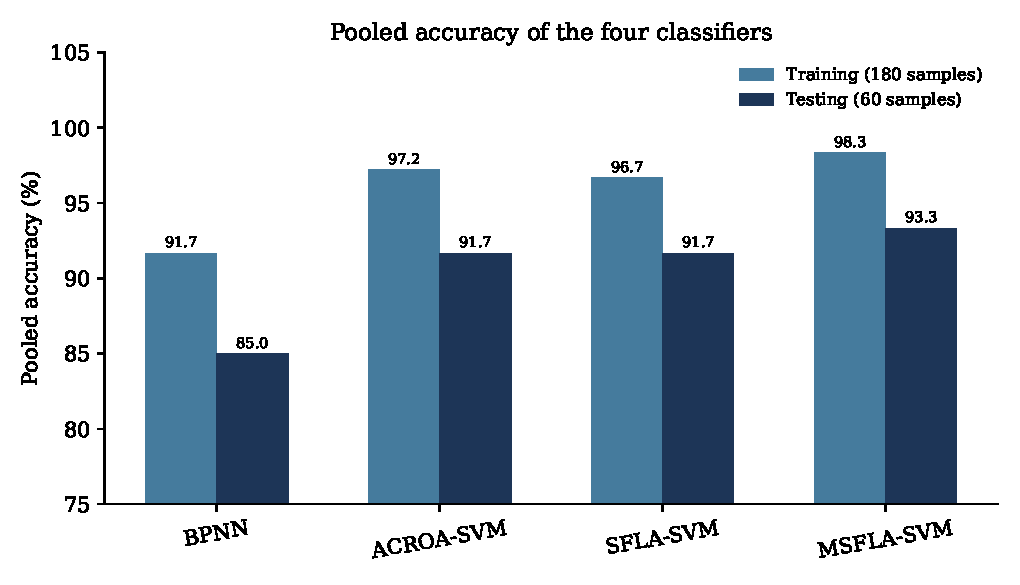
\includegraphics[width=0.82\textwidth]{pooled_accuracy.pdf}
\caption{Pooled training and test accuracy. The vertical gap inside each pair is the in-sample drop on \(60\) unseen vectors.}
\label{fig:pooled}
\end{figure}

The pooled test accuracies are \(85.0\%\) for the neural baseline, \(91.7\%\) for ACROA-SVM, \(91.7\%\) for SFLA-SVM, and \(93.3\%\) for MSFLA-SVM.
In counts, MSFLA-SVM labels \(56\) of the \(60\) test vectors correctly, the other two SVM searches label \(55\), and the neural baseline labels \(51\).
The modification of the leap is associated with one additional correct test vector relative to the unmodified leap and relative to the chemical-reaction search, and with five additional correct test vectors relative to the neural baseline.
Per state, MSFLA-SVM is never behind SFLA-SVM.
It ties SFLA-SVM on the healthy state (\(15/15\)), on the eccentric state (\(14/15\)), and on the pedestal state (\(13/15\)), and it labels one more sealing-ring vector correctly (\(14/15\) against \(13/15\)).
The entire pooled gain of the modification, on this test set, is that one sealing-ring vector.
Stating the result this way is more informative than stating only \(93.3\%\) against \(91.7\%\).

ACROA-SVM and SFLA-SVM land on the same pooled count by different per-class errors.
ACROA-SVM misses two eccentric vectors and one pedestal vector and one sealing-ring vector, in the sense that its correct counts are \(15\), \(13\), \(13\), and \(14\).
SFLA-SVM misses one eccentric vector, two pedestal vectors, and two sealing-ring vectors: correct counts \(15\), \(14\), \(13\), and \(13\).
The same number of errors is not the same error.
A maintenance decision that treats seal wear as more urgent than a mild eccentricity would prefer the ACROA pattern to the SFLA pattern even though the pooled rates match, and would prefer the MSFLA pattern to both because it keeps the ACROA seal-wear count and the SFLA eccentric count together.
The source does not publish the off-diagonal of the confusion matrix, so this paragraph accounts for misses per class and does not say which wrong label received them.

\subsection{Generalization drop}

The drop from pooled training accuracy to pooled test accuracy is a direct estimate of in-sample optimism:
\begin{equation}
\Delta = \mathrm{Acc}_{\mathrm{train}}-\mathrm{Acc}_{\mathrm{test}}.
\label{eq:drop}
\end{equation}
Table~\ref{tab:drop} evaluates \eqref{eq:drop} in percentage points and in counts.
The neural baseline drops \(6.67\) points, which is fourteen vectors of disagreement between the two rates' implied error counts (fifteen training errors out of \(180\), nine test errors out of \(60\)).
ACROA-SVM drops \(5.56\) points, SFLA-SVM drops \(5.00\) points, and MSFLA-SVM drops \(5.00\) points.
The modification does not enlarge the drop relative to the unmodified leap.
That fact matters because a search that found a higher training accuracy by memorizing the folds would usually pay for it on the test set.
MSFLA-SVM has both the highest training accuracy and the highest test accuracy, and its drop equals the drop of SFLA-SVM.
On a sample of this size the equality is one or two vectors, not a theorem.
It is still the right comparison to report, and it points in the direction the capacity argument of Chapter~\ref{ch:previous} predicts: the radial machines, all three of them, give up less accuracy when they leave the training sample than the neural baseline does.

\begin{table}[H]
\centering
\caption{Drop from pooled training accuracy to pooled test accuracy.}
\label{tab:drop}
\begin{tabular}{lrrr}
\toprule
Method & Training errors / 180 & Test errors / 60 & Drop (points) \\
\midrule
BPNN & 15 & 9 & 6.67 \\
ACROA-SVM & 5 & 5 & 5.56 \\
SFLA-SVM & 6 & 5 & 5.00 \\
MSFLA-SVM & 3 & 4 & 5.00 \\
\bottomrule
\end{tabular}
\end{table}

Per-class test means, averaged across the four methods as the source averages them, are \(96.667\%\) healthy, \(90\%\) eccentric, \(85\%\) pedestal, and \(90\%\) sealing-ring.
The healthy class is recognized by every SVM variant without a test error.
The pedestal class contributes two test errors to each SVM variant and three to the neural baseline.
The source's explanation is the one the signatures support.
The raw pedestal record is restricted by component resonance and by field interference, so the high-order coordinates that should describe the fault are also the coordinates the interference occupies.
VWC does not include a spatial filter or a coherence test against a second sensor that could reject a site tone.
The residual confusion is therefore a property of the measurement, and a better leap does not remove it.
MSFLA-SVM ties the other SVM methods at \(13/15\) on this class.
The open improvement the source itself names, better signal conditioning and less interference, sits in front of \(\Phi\), not inside the leap.

\subsection{How large the differences are}

A honest estimate states a difference in the unit the experiment controls, which is the labeled vector.
On the test set:
\begin{itemize}
\item MSFLA-SVM against BPNN: five vectors, \(56\) against \(51\), pooled rates \(93.333\%\) against \(85.000\%\).
\item MSFLA-SVM against ACROA-SVM: one vector, \(56\) against \(55\).
\item MSFLA-SVM against SFLA-SVM: one vector, \(56\) against \(55\), and that vector is a sealing-ring case.
\item ACROA-SVM against SFLA-SVM: zero vectors in the pooled count, with a different distribution across classes.
\end{itemize}
A five-vector gap against the neural baseline, on a sixty-vector test set, is large enough to be visible state by state: the neural baseline is behind on every state.
A one-vector gap between two global searches is the smallest nonzero gap the experiment can print.
It is consistent with the claim that the modified leap is not worse than the unmodified leap or the chemical-reaction search, and it is thin evidence for a claim that the modified leap is largely better.
The training table, where MSFLA-SVM leads by three vectors over SFLA-SVM and by two over ACROA-SVM, points the same way with a slightly larger count.
This paper reports both tables and does not promote the test gap of one vector into a percentage-point slogan detached from the denominator.

No confidence interval is published by the source, and none is fabricated here from an independence assumption the split may not obey.
If a reader assumes independent Bernoulli trials with success probability \(0.933\) and sixty trials, the standard deviation of the pooled accuracy is about \(\sqrt{0.933\cdot 0.067/60}\approx 0.032\), a little over three points, comparable to the gap between MSFLA-SVM and the neural baseline and larger than the gap between MSFLA-SVM and the other SVM searches.
The assumption is stronger than the evidence, because vectors from the same physical run are dependent.
The arithmetic is recorded only to show that the one-vector gap sits inside ordinary binomial variation and the five-vector gap sits at its edge.
A definitive ranking of the three searches would need a larger test set or a repeated split.

\subsection{What the estimate establishes}

The estimate establishes the following, and no more than the following.
\begin{enumerate}
\item The VWC vector, built from radial severity and from seven shaft-order coefficient amplitudes in three directions, separates the healthy pump from the three seeded faults well enough that a radial SVM labels at least \(55\) of \(60\) held-out vectors correctly.
\item The healthy state is linearly obvious in this vector for every SVM search: \(15\) of \(15\) test vectors, and \(45\) of \(45\) training vectors.
\item The eccentric state is the intensity fault.
Its severity is \(3.737\,\mathrm{mm/s}\) against \(1.051\,\mathrm{mm/s}\), and its test accuracy under MSFLA-SVM is \(14/15\).
\item The pedestal state is the shape fault and the hard fault.
Its severity is close to the healthy severity, its tangential energy moves to \(\tfrac12 f_{0}\), and every method, including the modified search, misses at least two of its fifteen test vectors.
\item On a shared VWC vector, the modified leap reaches a higher training count (\(177/180\)) and a higher test count (\(56/60\)) than the unmodified leap (\(174/180\) and \(55/60\)) and than the chemical-reaction search (\(175/180\) and \(55/60\)).
The test margin over each of those searches is one vector.
\item The backpropagation baseline, on the same vector, reaches \(165/180\) in training and \(51/60\) in testing.
The margin of MSFLA-SVM over this baseline is twelve training vectors and five test vectors, and the baseline's train-to-test drop is the largest of the four.
\end{enumerate}

\subsection{What the estimate does not establish}

The estimate does not establish a detection latency, because the records are labeled conditions rather than a timed evolution from healthy to faulty.
It does not establish performance at any speed other than \(960\,\mathrm{r/min}\), at any flow other than \(550\,\mathrm{m}^{3}/\mathrm{h}\), or under a mixture of two faults.
It does not establish which coordinate of the \(22\)-vector is necessary, because no ablation is published.
It does not establish the numerical pair \((C, g)\) that the leap returned, nor the population size, nor the number of shuffles.
It does not establish that db4 was the mother wavelet of the 2019 run; db4 is the wavelet of the illustrative energy figure and of the specification in Chapter~\ref{ch:methods}.
It does not establish a ranking of MSFLA against every published optimizer.
Particle swarm, genetic algorithm, and bee colony do not appear in the pump tables.
The related work reviewed in Chapter~\ref{ch:previous} shows that those searches are competitive on other machines.
A claim that the distance-weighted leap dominates them on this pump would be a new experiment.

The illustrative signals support none of the six positive statements above.
Those statements rest on the published severities, the published spectral reading, and the published counts.
The signals support only the narrower pedagogical claim that a record with the published severity and the published harmonic emphasis looks like Figure~\ref{fig:waves} and Figure~\ref{fig:spectra}, and that a db4 bank applied to such a record produces a nontrivial scale distribution, Figure~\ref{fig:energy}.

\subsection{Reading the result against the problem statement}

Section~\ref{sec:problem} asked for four things: a \(22\)-dimensional feature that carries intensity, scale, and shaft order; a leap that uses both leaders and that mutates locally; a build that makes the feature meaningful; and an estimate that respects the denominator of the test set.
The feature is specified in Section~\ref{sec:vwc} and is the common input of Table~\ref{tab:test}.
The leap is specified in Section~\ref{sec:svm} and is the unique difference between the SFLA column and the MSFLA column.
The build is specified in Section~\ref{sec:build}, and the arithmetic \eqref{eq:arith} shows that the clock matches the frequency family the feature samples.
The estimate is Table~\ref{tab:test} read in counts.
On those terms the pair of technologies does what the source claimed in direction and in magnitude: the modified search is the best of the four printed methods, the gain over the unmodified search is small, and the pedestal fault remains the open class.
The practical recommendation that follows is modest and precise.
Use the VWC vector rather than severity alone, because the pedestal fault is invisible to severity.
Use a radial SVM rather than the unconstrained neural baseline on a training set of \(180\) vectors, because the test drop is smaller and the test count is higher.
Use the modified leap in preference to the unmodified leap if the implementation cost is the same, and do not expect more than a vector or two on a test set of sixty.
Spend the next experimental effort on the interference in the pedestal records, which is where all four methods already agree that the present vector is weakest.

\subsection{Reproducibility notes}

A third party who rebuilds the system from this paper and from the source can match the following without access to the unpublished raw waveforms: the shaft frequency, the blade-pass frequency, the record duration, the Fourier resolution, the coefficient-domain Nyquist at level \(5\), the shapes of the two design matrices, every cell of the corrected test table, and every cell of the training table.
Matching the classifier byte for byte additionally requires the raw records, the mother wavelet, the integrator, the split, the search box actually used, and the population schedule.
The source states that the data are available from the corresponding authors on request.
Until those records are in hand, the illustrative figures of this paper should stay captioned as illustrations, and the tables of this chapter should stay captioned as a reading of the published counts.
That division is the reproducibility condition of the estimate.

\subsection{Error budget of the measurement chain}
\label{sec:budget}

The classification counts already include every error the chain actually made.
A separate budget is still useful, because it shows which contributions are large enough to move a feature and which are not.
Start from the sensor.
The B\&K~4321 charge sensitivity is stated as \(9.8\,\mathrm{pC/g}\) within \(\pm 2\%\).
A two-percent scale error multiplies every acceleration sample on that axis by a factor between \(0.98\) and \(1.02\).
Severity, being an RMS of a quantity linear in acceleration, inherits the same relative error:
\begin{equation}
\frac{\Delta\mathrm{VIB}}{\mathrm{VIB}}\approx 0.02.
\label{eq:senserr}
\end{equation}
On the healthy severity of \(1.051\,\mathrm{mm/s}\) this is about \(0.021\,\mathrm{mm/s}\).
On the eccentric severity of \(3.737\,\mathrm{mm/s}\) it is about \(0.075\,\mathrm{mm/s}\).
The gap between healthy and pedestal severities is \(1.161-1.051=0.110\,\mathrm{mm/s}\).
A two-percent calibration error is a fifth of that gap on the healthy reading and is smaller than the gap.
It does not by itself explain a confusion between those two states, and it is negligible beside the factor \(3.56\) that separates the eccentric state from the healthy state.
After the train-only normalization \eqref{eq:norm}, a pure scale error that is constant for the whole campaign is absorbed into \(u^{(j)}\) and \(v^{(j)}\) of the severity coordinate, provided the same sensor and the same gain are used for every record.
A scale error that changed between the training days and the test days would not be absorbed.
The source does not report a recalibration, and the budget assumes the gain was held fixed.

The acquisition card states a DC accuracy of \(\pm 0.1\%\) of full-scale range.
On the \(\pm 10\,\mathrm{V}\) range this is \(10\,\mathrm{mV}\).
On the \(\pm 100\,\mathrm{mV}\) range it is \(0.1\,\mathrm{mV}\).
Which range was selected is not printed.
The time-domain plots show accelerations of roughly \(7\) to \(9\,\mathrm{m/s}^{2}\), about one \(g\).
At \(9.8\,\mathrm{pC/g}\) that motion produces about \(10\,\mathrm{pC}\) at the peaks.
The voltage that results is the charge divided by the amplifier's feedback capacitance, a setting the source also does not print.
The relevant statement the budget can still make is comparative.
A full-scale error of \(0.1\%\) is twenty times smaller than the sensor's \(2\%\) sensitivity tolerance, so on any range that actually uses a reasonable fraction of its bits the card is not the leading scale error.
Quantization at, for example, a \(16\)-bit converter on a range matched to a few \(g\) sits well below both.
The chain is sensor-limited for amplitude, and it is clock-limited for frequency.

Clock error moves the orders in Table~\ref{tab:bins}.
A sampling-rate error of \(\varepsilon\) moves every apparent frequency by the same relative amount.
The widest order, \(6f_{0}=96\,\mathrm{Hz}\), moves by \(96\varepsilon\).
The half-order acceptance window specified for this exposition is \(4\,\mathrm{Hz}\).
Keeping the true \(6f_{0}\) inside that window requires
\begin{equation}
96\,\abs{\varepsilon}<4
\qquad\Rightarrow\qquad
\abs{\varepsilon}<0.042,
\label{eq:clock}
\end{equation}
a four-percent clock, which any PXI timebase meets by a wide margin.
The binding frequency constraint is not the clock.
It is the mechanical speed.
A one-percent speed drift, already discussed as an envelope of the method, moves \(6f_{0}\) by about \(1\,\mathrm{Hz}\), still inside the window, and moves the supply-to-\(3f_{0}\) gap from \(2.00\,\mathrm{Hz}\) to either \(1.52\,\mathrm{Hz}\) or \(2.48\,\mathrm{Hz}\) according to the sign.
The \(1.22\,\mathrm{Hz}\) bin can still hold them apart.
A speed that was only nominally \(960\,\mathrm{r/min}\), and that wandered by several percent inside a record, would broaden every order and would raise the pedestal and seal-wear confusion first, because those states are identified by which order is largest rather than by a large severity.
The source states a single speed.
The budget treats residual speed wander as an unquantified contribution inside the pedestal errors, not as a number the tables support.

Aliasing is the contribution the budget cannot bound from the printed table.
The sensor responds to \(12\,\mathrm{kHz}\) and the converter samples at \(10\,\mathrm{kHz}\), so energy between \(5\) and \(12\,\mathrm{kHz}\) folds into \(0\) to \(5\,\mathrm{kHz}\) unless an analog filter stops it.
Folded energy lands preferentially in the fine wavelet levels, and it can change which level wins \(k^{\star}\).
If the winning level moves, the coefficient rate changes and the amplitudes \eqref{eq:samples} are read on a different series.
The source plots show \(d_{5}\) winning for the displayed records, which is evidence that, on those records, the mid band carried the energy, and it is not evidence that an anti-alias filter was present.
A repetition of the build should state the filter cutoff next to the \(10\,\mathrm{kHz}\) clock.
Until that cutoff is known, high-frequency folding remains an open term in the budget and a candidate contributor to the two pedestal test errors that every SVM method still makes.

Interference tones that the order sampler does not aim at --- the reported crosstalk at \(28\), \(34\), and \(38\,\mathrm{Hz}\) under the eccentric fault, and the supply line at \(50\,\mathrm{Hz}\) --- are rejected by the sampler's narrow windows and are not rejected by the wavelet energy that chooses the level.
They can change \(k^{\star}\) without entering \(\vect{x}\) as their own coordinates.
That indirect path is the reason a clean mechanical spectrum and a clean scale choice are both part of signal conditioning, which is the improvement the source itself defers to future work.
The budget's conclusion is short.
Calibration and quantization are too small to explain the published confusions.
Speed error at the one-percent level is tolerable for the order windows.
Unfiltered high-frequency energy and in-band interference are large enough, in mechanism, to move the pedestal features, and they are exactly the mechanisms named in the source discussion of that class.

\subsection{An operating procedure for one labeled record}
\label{sec:procedure}

The build is reproducible as a sequence even where some numerical settings remain those of the original run.
One labeled record, from the command to start the pump through the row that enters \(\vect{X}\), is the following procedure.
It is the system of Section~\ref{sec:build} written as steps an operator can tick, not as a new experiment.
\begin{enumerate}
\item Set the loop to the duty in Table~\ref{tab:rig}: \(960\,\mathrm{r/min}\), \(550\,\mathrm{m}^{3}/\mathrm{h}\), \(3\,\mathrm{m}\) head, four-blade impeller, closed circuit.
Confirm \(f_{0}=16\,\mathrm{Hz}\) from a tachometer or from the once-per-revolution line before any fault label is trusted.
\item Install the fault for this record, or install none.
Eccentric axle: displace the balance weight and record the mass and the radius, even though the classifier never sees those two numbers, because a later reader of the severity \(3.737\,\mathrm{mm/s}\) will want them.
Pedestal: seed the bearing defect the campaign has defined and confirm that the pedestal is the vibrating part under the sensor.
Seal wear: use the worn ring the campaign has defined and confirm that the impeller is not rubbing.
Do not combine two of these in one record.
The label set is a partition.
\item Mount the triaxial charge accelerometer on the casing.
Note the direction that will be called radial, because that direction supplies the single severity coordinate.
Check that the charge cables and the amplifier gains are the same ones used for the records already in the training matrix.
\item Set the converter to \(10\,\mathrm{kHz}\), confirm the anti-alias cutoff is below \(5\,\mathrm{kHz}\), and arm a capture of at least \(8192\) samples on all three axes after the pump has been at speed long enough for the flow to be steady.
Store the three series and the tachometer reading with the state label.
\item Compute radial severity by the campaign's stated integrator and by \eqref{eq:vibdisc}.
Run the eight-level db4 bank on each axis, select \(k^{\star}\) by \eqref{eq:kstar} with the finer level winning a tie, and sample the seven orders of \eqref{eq:ordersexact} from the coefficient power spectrum \eqref{eq:cps} through the frequency map \eqref{eq:fmap}.
Refuse any order above the coefficient Nyquist of the winning level.
\item Assemble \eqref{eq:x22}.
If the row is a training row, update nothing about scaling until the full training matrix exists, then fit \eqref{eq:norm}.
If the row is a test row, apply the training ranges already stored.
Do not refit them.
\item When \(180\) training rows are in hand, run the modified leap inside the box \eqref{eq:box} with fitness \eqref{eq:fitness}, retrain the six binary machines on all \(180\) rows at the returned pair, and only then label the \(60\) test rows by vote.
Log the six items of Section~\ref{sec:cost}.
\end{enumerate}
Steps 1--4 are the rig.
Steps 5 and 6 are VWC.
Step 7 is MSFLA-SVM.
A baseline replaces step 7 and does not replace steps 1--6.
That separation is what makes Table~\ref{tab:test} a comparison of classifiers on one feature.

The procedure also says what the operator does not do.
The operator does not choose \(C\) and \(g\) by hand after looking at the test labels.
The operator does not drop the pedestal records because they are harder.
The operator does not lengthen the test set by moving training rows across the split after the search has run.
Each of those moves would raise a number in Table~\ref{tab:test} and would destroy the estimate.
The published counts are informative because, as far as the source text shows, none of those moves was made.

\subsection{The estimate in the unit the experiment controls}
\label{sec:unit}

Table~\ref{tab:errors} restates the published result as error counts, which is the unit in which a one-vector gap is not asked to look like a percentage-point discovery.
Training errors are out of \(180\).
Test errors are out of \(60\).
The per-class test errors follow by subtracting the correct counts of Table~\ref{tab:test} from \(15\).

\begin{table}[H]
\centering
\caption{Error counts. Training errors are out of \(180\) pooled vectors. Test errors are out of \(60\) pooled vectors, and the four class columns are out of \(15\).}
\label{tab:errors}
\begin{tabular}{lrrrrrr}
\toprule
Method & Train & Test & Normal & EAF & BPF & SRWF \\
\midrule
BPNN & 15 & 9 & 2 & 2 & 3 & 2 \\
ACROA-SVM & 5 & 5 & 0 & 2 & 2 & 1 \\
SFLA-SVM & 6 & 5 & 0 & 1 & 2 & 2 \\
MSFLA-SVM & 3 & 4 & 0 & 1 & 2 & 1 \\
\bottomrule
\end{tabular}
\end{table}

Read across the test columns, the modified search matches the better of the other two searches in every state: it matches SFLA-SVM on the eccentric axle (one error), matches both SVM searches on the pedestal (two errors), matches ACROA-SVM on seal wear (one error), and matches every SVM search on the healthy state (no error).
It does not create a new kind of success on the pedestal.
It collects, in one rule, the per-class results that the other searches hold only separately.
That is a fair description of a one-vector pooled gain, and it is the description this estimate keeps.

Read down the pedestal column, no method is in single digits of a different kind: the best pedestal result on the test set is two errors out of fifteen, which is \(13/15\).
The training pedestal column of Table~\ref{tab:train} is consistent with the same ranking.
MSFLA-SVM misses two of forty-five pedestal training vectors, and every other method misses more.
The feature, not the leap, is saturated on this class.
Further optimization of \((C, g)\) can rearrange one error among the easier classes, which is what the sealing-ring column shows, and it has not been observed to buy a pedestal test vector.

The practical statement that closes the estimate is therefore a statement about effort.
On this rig, with this sample, the VWC vector plus a radial SVM already carries the diagnosis from the neural baseline's nine test errors to five.
The modified leap carries it from five to four, by avoiding one seal-wear error that the unmodified leap makes and one eccentric error that the chemical-reaction search makes.
The two pedestal errors that remain are the next experiment: a second sensor, a stated anti-alias filter, or a conditioning step aimed at the site tones, scored on a new split.
They are not a reason to discard the twenty-two coordinates or the leap that reads them.
They are the part of the problem the published counts show is still open.

